\documentclass[12pt]{article}
\usepackage{graphicx}
\usepackage[utf8]{inputenc}
\usepackage{amsmath}
\usepackage[top=30mm,bottom=30mm,left = 30mm , right = 30mm]{geometry}
\usepackage{xcolor}
\usepackage{wrapfig}
\usepackage{caption,subcaption}
\usepackage{hyperref}
\hypersetup{colorlinks,	citecolor=black, filecolor=black, linkcolor=black, urlcolor=black}
\usepackage{setspace}
\usepackage{pdfpages}
\usepackage{cite}
\graphicspath{{../Results/}}

\title{Autocorrelation in Weather}
\author{Pablo Lechon}
\date{}

\begin{document}

	\maketitle	
	\section{Introduction}
		The goal in this practical is to write an r script that helps answer the question: \textit{are temperatures of one year significantly correlated with the next year (successive years), across years in a given location?}\\
		For this, we calculate the correlation between $n - 1$ pairs of years, where $n$ is the total number of years. note that one cannot use the standard p-value calculated for a correlation coefficient, because measurements of climatic variables in successive time-points in a time series (successive seconds, minutes, hours, months, years, etc.) are \textit{not independent}.

	\section{Data}
%		We first load the data with the comand \verb|load(filename, envir = globalenv())|, which consists of two columns: Year and Temperature. A quick plot to visualize these data can be seen in \ref{temp}//
		\begin{figure}[h]
			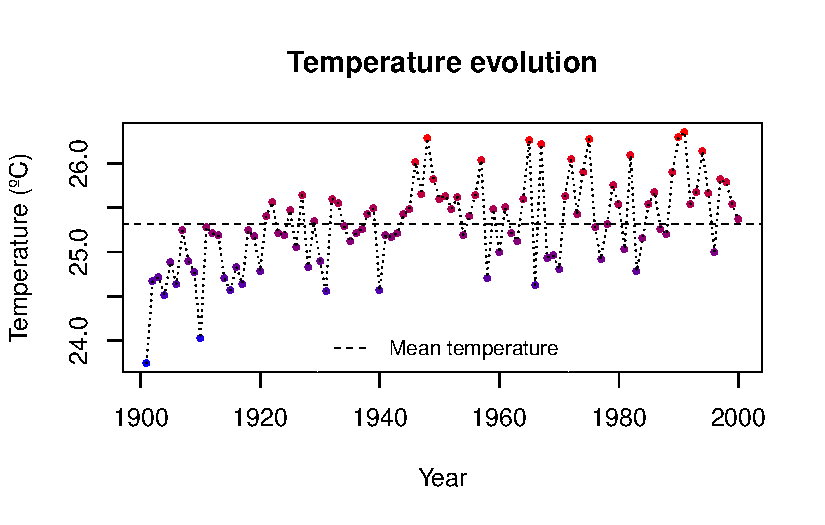
\includegraphics{temp_evolution.pdf}		
			\centering
			\caption{Temperature time series. Redder indicates wormer. A dasshed line connects the points for better visualization}
			\label{temp}
		\end{figure}

\end{document}